\documentclass[12pt,english,brazil,a4paper,utf8,oneside]{utfpr-tcc}

% carrega o arquivo configuracoes.tex que contém os pacotes e comandos Latex.
%
% Esse arquivo conterá pacotes e comandos utilizados na monografia
%
% Observação - devido a um erro do sharelatex foi necessário colocar na raiz do projeto os seguintes arquivos:
% gcnumparser.sty, fcprefix.sty, fmtcount.sty, fc-poruges.def, fcportuguese.def.
% Tal problema foi relatado em: https://github.com/nlct/fmtcount/issues/26
% Quando o sharelatex corrigir o problema acredito que podemos remover esses arquivos do projeto. At. Luiz Arthur.
%

% Este comando não é necessário: utilizei apenas para deixar o latex2rtf
% feliz (e descobrir a codificação do texto).
\usepackage[utf8]{inputenc}

% Suporte a figuras e subfiguras
\usepackage{graphics}
\usepackage{subfigure}

% Suporte a tabelas (principalmente do cronograma)
\usepackage{tabularx}
\usepackage{multirow}
\usepackage{array}
\usepackage{tabularx}
\usepackage{colortbl}
\usepackage{hhline}
\usepackage{xcolor}


% better tables
\usepackage{booktabs}

% frame box
\usepackage{mdframed}

% Escalar fontes para redimencionar, por exemplo tabelas
\usepackage{scalefnt}

% Algoritmos.
\usepackage{algorithm,algorithmic}

\usepackage[alf]{abntex2cite}

% the table's styles
\usepackage{booktabs}

% Elementos geralmente utilizados na tabela do cronograma
\newcommand{\fullcell}{\multicolumn{1}{>{\columncolor[gray]{0.5}}c}{}}
\newcommand{\fullcellline}{\multicolumn{1}{>{\columncolor[gray]{0.5}}c|}{}}
\newcommand{\mc}[3]{\multicolumn{#1}{#2}{#3}}
\newcommand{\y}{\rule{8pt}{4pt}}
\newcommand{\n}{\hspace*{8pt}}

% Define o caminho das figuras
\graphicspath{{images/}}

%% Configuração de glossário
\usepackage[portuguese]{nomencl}
\usepackage[nogroupskip,acronym,nomain,nonumberlist,nopostdot,nohypertypes={acronym}]{glossaries}

\makenoidxglossaries

% para siglas em português
\newcommand{\sigla}[2]
{
 \newglossaryentry{#1}{
  name=#1,
  description={#2},
  first={#2 (#1)},
  long={#2}
 }  
}

% para siglas de língua estrangeira, nessas a descrição longa fica em itálico.
\newcommand{\siglaIt}[2]
{
 \newglossaryentry{#1}{
  name=#1,
  description={\textit{#2}},
  first={\textit{#2} ({#1})},
  long={\textit{#2}}
 }  
}

% --- Estilos para apresentação de Código ----- %
\usepackage{listings}
\lstset{escapechar=§}
\lstloadaspects{formats}

\lstset{
	aboveskip=0cm,
	stringstyle=\ttfamily,
	showstringspaces = false,
	basicstyle=\scriptsize\ttfamily,
	commentstyle=\color{gray!45},
	keywordstyle=\bfseries,
	ndkeywordstyle=\bfseries,
	identifierstyle=\ttfamily,
	numbers=left,
	numbersep=15pt,
	numberstyle=\tiny,
	numberfirstline = false,
	breaklines=true
}

\lstdefinelanguage{JavaScript}{
	keywords={typeof, new, true, false, catch, function, return, null, catch, switch, var, const, let, async, await, if, in, while, do, else, case, break, from},
	ndkeywords={class, export, boolean, throw, implements, import, this},
	sensitive=false,
	comment=[l]{//},
	morecomment=[s]{/*}{*/},
	morestring=[b]',
	morestring=[b]"
}

% Diff language
\usepackage{xcolor}
\definecolor{diffstart}{named}{lightgray}
\definecolor{diffincl}{named}{blue}
\definecolor{diffrem}{named}{red}

\lstset{
	aboveskip=0cm,
	stringstyle=\scriptsize,
	showstringspaces = false,
	basicstyle=\scriptsize\ttfamily,
	commentstyle=\color{gray!45},
	keywordstyle=\bfseries,
	ndkeywordstyle=\bfseries,
	identifierstyle=\ttfamily,
	numbers=left,
	numbersep=15pt,
	numberstyle=\tiny,
	numberfirstline = false,
	breaklines=true
}

\lstdefinelanguage{diff}{
    basicstyle=\scriptsize\ttfamily,
	morecomment=[f][\color{diffstart}]{@@},
	morecomment=[f][\color{diffincl}]{+\ },
	morecomment=[f][\color{diffrem}]{-\ },
	morestring=[b]',
	morestring=[b]",
	keywords={typeof, new, true, false, catch, function, return, null, catch, switch, var, const, let, async, await, if, in, while, do, else, case, break, from},		
	ndkeywords={class, export, boolean, throw, implements, import, this},
}
% --- Fim da Definição de Estilos para apresentação de Código ----- %
% carrega o arquivo constantes.tex que contém dados do curso/monografia que NÃO DEVEM ser alterados. 
%% Dados do curso que não precisam de alteração
\university{Universidade Tecnológica Federal do Paraná}
\universityen{Federal University of Technology -- Paraná}
\universityunit{Departamento Acadêmico de Computação}
\address{Campo Mourão}
\addressen{Campo Mourão, PR, Brazil}
\documenttype{Monografia}
\documenttypeen{Monograph}
\degreetype{Graduação}
% carrega o arquivo variaveis.tex que contém dados do acadêmico/monografia que DEVEM ser alterados.
%% Dados do curso. Caso seja BCC:
\program{Curso de Bacharelado em Ciência da Computação}
\programen{Undergradute Program in Computer Science}
\degree{Bacharel}
\degreearea{Ciência da Computação}
% Caso seja TSI:
% \program{Curso Superior de Tecnologia em Sistemas para Internet}
% \programen{Undergradute Program in Tecnology for Internet Systems}
% \degree{Tecnólogo}
% \degreearea{Tecnologia em Sistemas para Internet}


% Dados da disciplina. Escolha uma das opções e a descomente:
% TCC1:
\goal{Proposta de Trabalho de Conclusão de Curso de Graduação}
\course{Trabalho de Conclusão de Curso 1}
% TCC2:
% \goal{Trabalho de Conclusão de Curso de graduação}
% \course{Trabalho de Conclusão de Curso 2}


% Dados do TCC (precisa alterar)
\author{Daniel Venturini}  % Seu nome
\title{Estudo empírico sobre \textit{Break change} no ecossistema do NPM} % Título do trabalho
\titleen{An Empirical Study of Breaking Changes in the npm Ecosystem } % Título traduzido para inglês
\advisor{Prof. Dr. Ivanilton Polato} % Nome do orientador. Lembre-se de prefixar com "Prof. Dr.", "Profª. Drª.", "Prof. Me." ou "Profª. Me."}
\coadvisor{Prof. Dr. Igor Scaliante Wiese} % Nome do coorientador, caso exista. Caso não exista, comente a linha.
\depositshortdate{2019} % Ano em que depositou este documento

% Dados da ficha catalografica. Ela é opcional, mas é uma boa ideia inserí-la. Exemplos para geração (http://fichacatalografica.sibi.ufrj.br/)
\fichacatautor{}  % Nome conforme citado (ou seja, no formato "Sobrenome, Nome").
\fichacatbib{Biblioteca da UTFPR de Campo Mourão} % Não alterar
\fichacatpum{M488} % Código Cutter-Sanborn. Use a primeira letra do sobrenome seguido do número conforme as primeiras letras do sobrenome e a tabela http://www.amormino.com.br/cutter-sanborn/cutter1.html
\fichacatpalcha{} % Assuntos do trabalho. Cada item deve ser enumerado e separado por ponto: 1. xxx. 2. yyy. 3. zzz.
\fichacatpdois{} % Deixar em branco

% carrega o arquivo listaabreviaturas.tex que está dentro do diretório pretextual, esse arquivo contém as siglas utilizadas na monografia.
% quando a sigla for de língua portuguesa utilize \sigla{SIGLA}{Significado em português}
% quando a sigla for de língua estrangeira utilize \siglaIt{SIGLA}{Significado em Inglês}

\siglaIt{NPM}{Node Package Manager}
\siglaIt{HTTP}{HyperText Transfer Protocol}
\siglaIt{API}{Application Programming Interface}

% No texto quando for utilizar a sigla utilize os seguintes comandos:
%\acrlong{label} - acronimo/sigla longo
%\acrshort{label} - acronimo/sigla curta
%\Gls{TCP} - sigla com o significado primeiro em Maiusculo
%\GLS{TCP} - sigla com o significado tudo em MAIUSCULO
%\gls{TCP} - sigla com o significado tudo em minusculo % usando glossaries

\begin{document}
	
%\frontmatter
%\maketitle

% Dedicatória é opcional, para usar descomentar a linha a seguir e edite o arquivo pretextual/dedicatoria.tex
%\dedicate{Para minha mãe, para meu pai e para você...} % Opcional - descomentar para usar

% Agradecimento é opcional, para usar descomentar a linha a seguir e edite o arquivo pretextual/dedicatoria.tex
%\begin{agradecimentos}

agradeço agradeço agradeço agradeço agradeço agradeço agradeço agradeço  agradeço agradeço agradeço agradeço agradeço agradeço agradeço agradeço agradeço agradeço agradeço agradeço agradeço agradeço agradeço agradeço agradeço agradeço agradeço agradeço agradeço agradeço agradeço agradeço agradeço agradeço agradeço agradeço agradeço agradeço agradeço agradeço agradeço agradeço agradeço agradeço agradeço agradeço agradeço agradeço agradeço agradeço agradeço agradeço agradeço agradeço agradeço agradeço agradeço agradeço agradeço agradeço agradeço agradeço agradeço agradeço agradeço agradeço agradeço agradeço agradeço agradeço agradeço agradeço 

\end{agradecimentos} % Opcional - descomentar para usar

% carrega o arquivo resumo.tex que está dentro do diretório pretextual, esse arquivo deve conter o resumo da monografia.
%\begin{resumo}
%Elemento obrigatório, constituído de uma sequência de frases concisas e objetivas, em forma de texto.  Deve apresentar os objetivos, métodos empregados, resultados e conclusões.  O resumo deve ser redigido em parágrafo único, conter no máximo 500 palavras e ser seguido dos termos representativos do conteúdo do trabalho (palavras-chave).

% TODO: se possível, escreva um resumo estruturado. Para TCC 1, o resumo estruturado teria os seguintes elementos:
\textbf{Contexto:} o \textit{npm} é largamente utilizado e é o maior repositório para uma dada linguagem. Os pacotes hospedados no \textit{npm} dependem um dos outros, criando uma rede de interconectividade entre eles. Entretanto, os provedores evoluem independentemente dos seus clientes e, por vezes, introduzem alterações que podem causar um comportamento inesperado nos clientes. Essas alterações são as \textit{breaking changes} e se tornam um problema quando os clientes as recebem, mas não deveriam receber.\\
\textbf{Objetivo:} este trabalho propõe mensurar e categorizar as \textit{breaking changes} e analisar como os clientes se recuperam delas.\\
\textbf{Método:} de uma amostra dos pacotes do \textit{npm}, copiá-los localmente, resolver a versão dos seus provedores para a última versão disponível no momento da \textit{release} do cliente. Posteriormente, executar o pacote através dos \textit{scripts npm install/npm test}. Então, para cada \textit{release} do cliente que resultou em erro, verificar no código da \textit{release} e no repositório do provedor para confirmar se o erro foi causado pelo provedor, sendo então uma \textit{breaking change}.\\
% \textbf{Resultados esperados:} 
% ou, para TCC 2:
% \textbf{Contexto:} \\
% \textbf{Objetivo:} \\
% \textbf{Método:} \\
% \textbf{Resultados:} \\
% \textbf{Conclusões:}

% Palavras-chaves, separadas por ponto (tente não definir mais do que cinco)
\palavraschaves{\textit{npm}. \textit{Breaking change}. Versionamento Semântico. Dependências}
\end{resumo}
% carrega o arquivo abstract.tex que está dentro do diretório pretextual, esse arquivo deve conter um resumo escrito na linguá inglesa para a monografia.
%% Caso seja TCC 2, precisa traduzir o resumo e as palavras-chaves para inglês:
\begin{abstract}
PUT THE ABSTRACT HERE...

% \textbf{Context:}
% \textbf{Objective:}
% \textbf{Method:}
% \textbf{Results:}
% \textbf{Conclusions:}

% Palavras-chaves em inglês, separadas por ponto.
% \keywords{}
\end{abstract}

% Listas (opcionais, mas recomenda-se a partir de 5 elementos)
%\listoffigures
%\listoftables
%\listofacronyms
%\printnoidxglossaries

% Sumário
%\tableofcontents

%\mainmatter

% Capítulos da monografia:
%\chapter{Introdução}
\label{cap:introducao}

O \textit{Node Package Manager} (\textit{npm}) é um gerenciador de pacotes para o \textit{Node.js} que possui um \textit{website}\footnote{https://npmjs.org}, no qual se pode consultar os pacotes, e um registro\footnote{http://registry.npmjs.org/}, no qual os pacotes publicados são armazenados. Lançado em 2009, seu principal objetivo é facilitar o compartilhamento de códigos escritos em \textit{JavaScript} -- além de outras linguagens de programação. Atualmente, o \textit{npm} ocupa a posição de maior repositório\daniel{ou registro?} para uma dada linguagem, com mais de 1 milhão de pacotes.\footnote{http://www.modulecounts.com} O \textit{npm} é um dos que impulsionaram o \textit{JavaScript} a se tornar um ecossistema completo, com pacotes, \textit{frameworks}, aplicativos \textit{mobiles}, aplicativos \textit{web} entre outros \cite{introduction:npm} e também,  97\% dos aplicativos \textit{web} são oriundos do \textit{npm}.\footnote{https://blog.npmjs.org/post/180868064080/this-year-in-javascript-2018-in-review-and-npms}

O \textit{npm} estimula o compartilhamento de código entre os pacotes e, por causa disso, contém o maior número de dependências entre os pacotes \cite{teorical_reference:npm_2}. Nesse cenário, o termo cliente refere-se àquele pacote que depende de outro pacote para executar, e o termo provedor refere-se àquele pacote que provê recursos para os seus cliente, conforme definidos na Seção \ref{ref-teo:prov_clie}. Assim, como muitos pacotes estão dependendo mutuamente, há uma rede que interconecta os pacotes, e quando há um erro em algum provedor, um grande número de clientes podem ser afetados. Foi exatamente isso que ocorreu através de um 


pacote chamado \textit{left-pad}.\footnote{https://blog.npmjs.org/post/141577284765/kik-left-pad-and-npm} Esse pacote foi removido do \textit{npm} por seu desenvolvedor e impactou milhares de outros pacotes em apenas 2.5 horas, incluindo pacotes renomados como o \textit{babel}\footnote{https://github.com/babel/babel} e o \textit{atom}\footnote{https://github.com/atom/atom} que propagaram essa quebra de dependência para seus clientes. Assim, problemas de comunicação entre os pacotes realmente ocorrem no ecossistema do \textit{npm} e por isso esse foi escolhido como estudo de caso, devido à rede de interconectividade entre os pacotes.

Um defeito que causa problemas de comunicações entre os pacotes são as \textit{breaking changes}, descritas na Seção \ref{ref-teo:breaking_change}. Uma \textit{breaking change} é uma alteração no provedor que o torna incompatível com as suas versões anteriores \cite{intro:break_change}, fazendo com que seus clientes tenham um comportamento indesejado. Um exemplo de \textit{breaking change} ocorreu na \textit{release optipng@0.2.0} na qual o método \textit{OptiPng.getBinaryPath} foi renomado para \textit{OptiPng.getBinPath}.\footnote{https://github.com/papandreou/node-optipng/compare/v0.1.1...v0.2.0\#diff-366460cd3c3170c9c84340631e6f8e4fL22-R19} Porém, o método foi renomeado por engano e a \textit{release} errônea foi publicada em uma versão \textit{minor} -- nível de versão do Versionamento Semântico, especificado na Seção \ref{ref-teo:semver} --, fazendo com que todos os clientes que tinham acesso àquele método não tivesse mais. Assim, o código \ref{cod:bc:optipng} executa normalmente com o \textit{optipng@0.1.1}, mas ao atualizar para o \textit{optipng@0.2.0}, esse código sofre uma \textit{breaking change} -- o que não deveria acontecer com uma \textit{release minor}.

\begin{lstlisting}[style=Javascript, label=cod:bc:optipng, caption={Código que sofre \textit{breaking change} do \textit{optipng}}]
var OptiPng = require('optipng');
var cb = {apply: () => {}};
OptiPng.getBinaryPath(cb);
\end{lstlisting}

Apesar de ser um erro facilmente detectável, esse foi consertado somente após 34 dias, conforme mostra a Figura \ref{fig:bc_optipng}. Esta correção foi realizada em um \textit{commit}\footnote{https://github.com/papandreou/node-optipng/commit/a155f2b078224be18367847bbcbd3df3c379deea} no qual o desenvolvedor comentou que a renomeação do método ocorreu por engano.

\begin{figure}
    \centering
    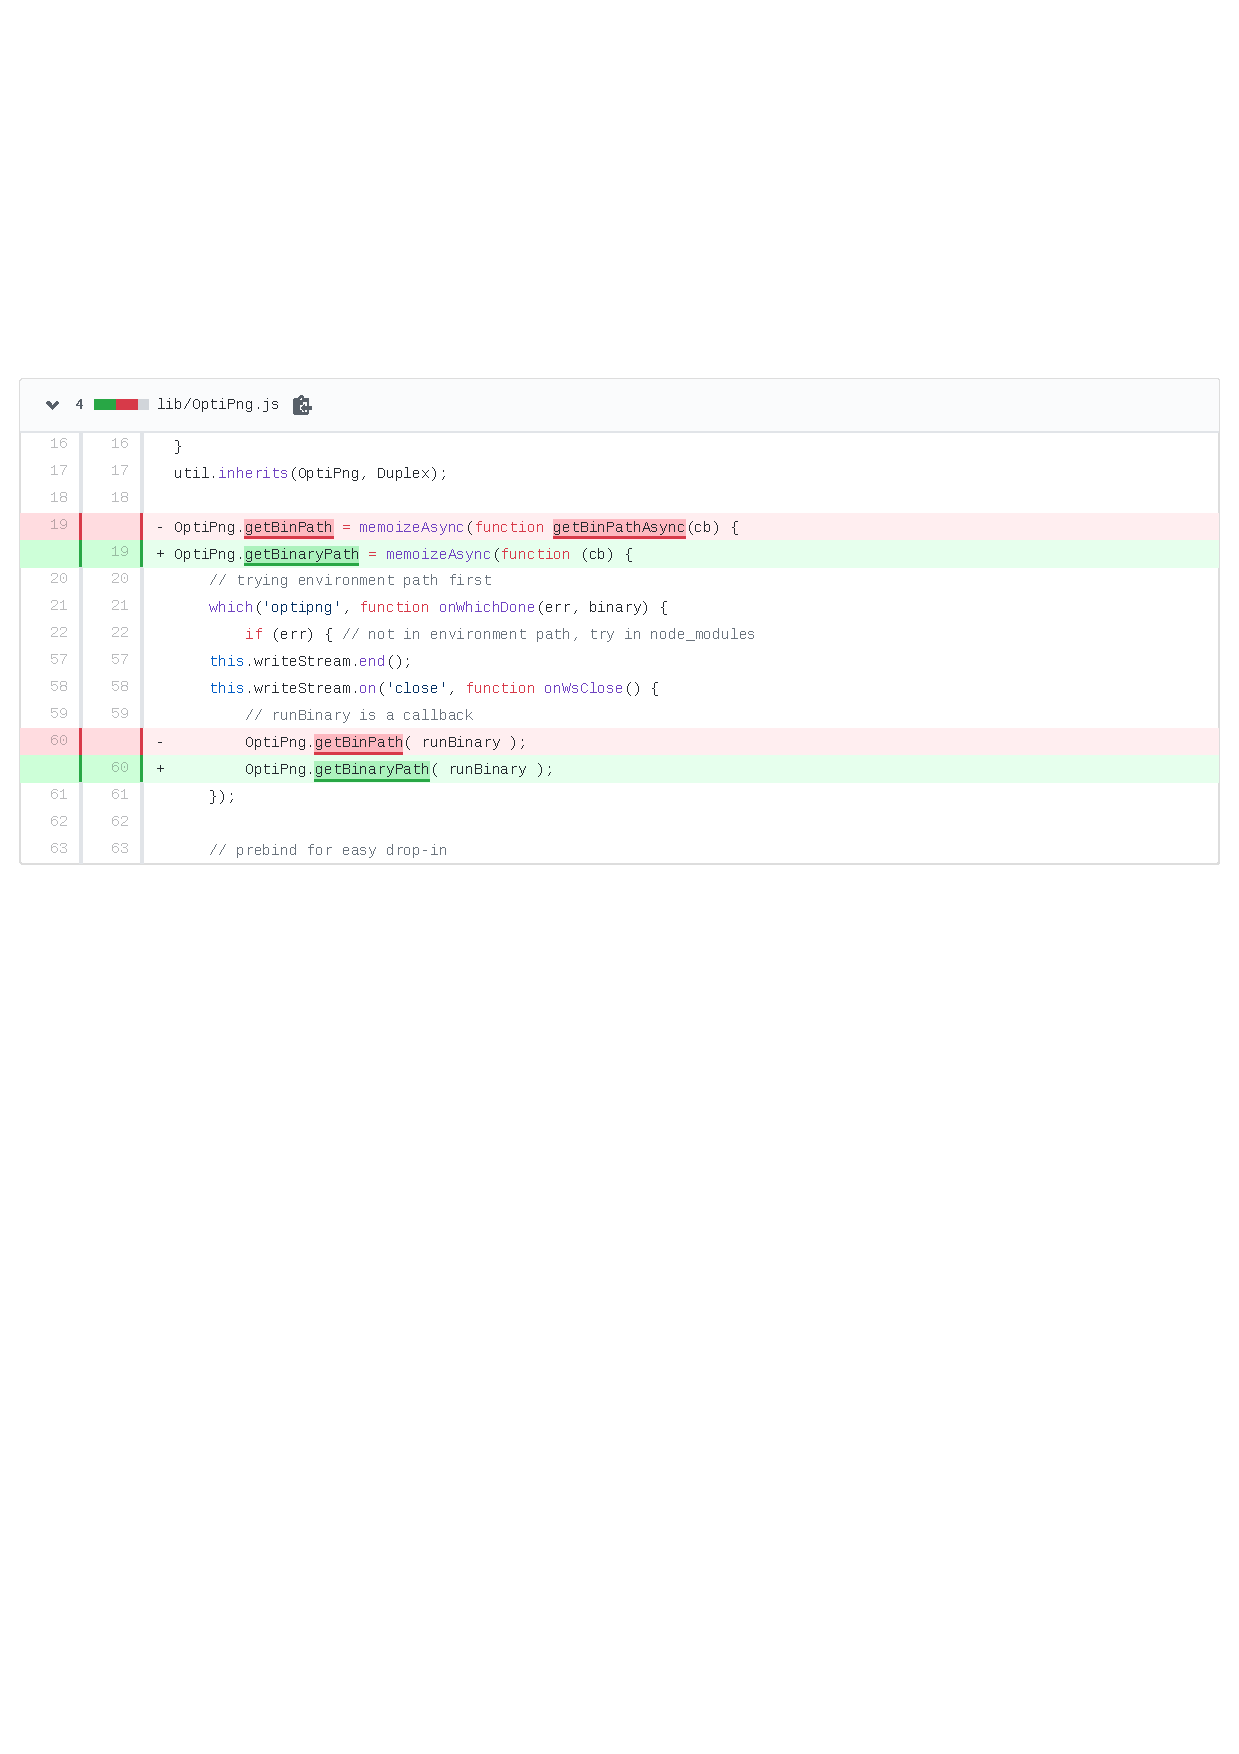
\includegraphics[scale=0.65]{figuras/bc_example.pdf}
    \caption{\textit{Commit} que corrigiu a \textit{breaking change}}
    \label{fig:bc_optipng}
\end{figure}{}

Alterações no código que causam \textit{breaking change} devem ser introduzidas em \textit{releases} versionadas com o incremento do nível \textit{major}, seguindo as especificações do Versionamento Semântico, definidos na Seção \ref{ref-teo:semver}. Assim, um cliente pode especificar se deseja ou não receber as \textit{releases} que contêm \textit{breaking change}. Entretanto, pesquisas relacionadas mostram que as \textit{breaking changes} são introduzidas erroneamente pelos provedores, assim, impactando os clientes. \citeonline{teorical_reference:bc_1} constatou que 9\% das \textit{releases} dos três pacotes com mais dependentes no \textit{npm} introduziram \textit{breaking changes} indevidamente e \citeonline{noregrets2018} apresentou uma ferramenta para detecção de \textit{breaking changes} e também constatou que 9\% das \textit{releases} introduziram \textit{breaking changes} quando não deveriam introduzir.
\daniel{Esses são os que eu coloquei nos trabalhos relacionados}

Além de quantificar as \textit{breaking changes} no ecossistema do \textit{npm}, este trabalho apresenta uma proposta para categorizar essas \textit{breaking changes} e verificar como os clientes se recuperam. Para isso, foi utilizado uma amostra representativa dos clientes no \textit{npm} e, para cada uma de suas \textit{releases}, foi verificado se houve alteração nas \textit{releases} que os clientes aceitavam dos provedores. Então, as versões dos provedores foram resolvidas para a última versão disponível até momento da publicação da \textit{release} do cliente e as \textit{releases} foram executadas através dos \textit{scripts npm install/npm test}. Após, foi feita uma análise manual no código das \textit{releases} que resultaram em erro para confirmar se o erro se tratava de uma \textit{breaking change} ou não. Por fim, foi feita uma análise nos repositórios dos provedores que introduziram as \textit{breaking change} para recuperar informações, tais como, tipo de \textit{breaking change}, tempo que levou até ser consertada, o nível da versão que a \textit{breaking change} foi introduzida/consertada.

Desse modo, o Capítulo \ref{cap:ref-teorico} contém a descrição de todos os termos utilizados ao longo desse trabalho. O Capítulo \ref{cap:qp} contém a motivação e o método para cada uma das questões de pesquisa. O Capítulo \ref{cap:metodologia} descreve sobre a manipulação dos dados que serão utilizados nessa pesquisa\daniel{serão ou foram?}. Por fim, o Capítulo \ref{cap:cronograma} apresenta o cronograma previsto das atividades faltantes para terminar esse trabalho.

% isso estava nos results
%\filipe{o erro sempre se manifesta no cliente, acho que o lance é que você consegue identificar se o erro foi proveniente de uma chamada a uma função do provedor ou do próprio cliente (ou algum outro provedor que não interessa à análise).}

%\filipe{breaking change (defeito no provedor) vs. manifestação da breaking change (manifestação do defeito do provedor no cliente)}
%\chapter{Conceitos}
\label{cap:conceitos}

Descreva os conceitos necessários para que o leitor entenda o seu trabalho (referencial teórico). 

Exemplo, se o seu trabalho é a respeito de banco de dados e redes você pode descrever conceitos a respeito desses assuntos ou de assuntos que ajudem ao leitor a entender a sua proposta/metodologia.

%---------------------------------------------------%
\section{Exemplo de uso de Equação}
\label{cap:conceitos:sec:usando:equacoes}

O valor mensurado do tráfego de bytes considerando todos os níveis da hierarquia de memória ($Q_{total}$) é calculado usando a Equação \ref{equ:roofline:qtotal}.

\begin{equation}\label{equ:roofline:qtotal}
Q_{total} = Q_{L1} + Q_{L2} + Q_{LLC} + Q_{MEM}
\end{equation}

%---------------------------------------------------%
\section{Usando Código}
\label{cap:conceitos:sec:usando:codigo}

Se for necessário apresentar a ideia de um Algoritmo~\ref{alg:decisao-001} em pseudocódigo...

\begin{algorithm}[H]
	\caption{Meu algoritmo}
	\label{alg:decisao-001}
	\begin{algorithmic}[1]
		\STATE $\textbf{INPUT:}*better\_device\_index$
		\STATE $\textbf{OUTPUT:} *better\_device\_index, offload\_decison$
		\STATE $offload\_decision \leftarrow true$
		\IF{($offload\_decision \leftarrow \textbf{RM\_check\_all\_eventsets\_was\_collected(})$)}
		\STATE $oi \leftarrow \textbf{RM\_get\_operational\_intensity}()$
		\STATE $better\_device\_index \leftarrow \textbf{RM\_get\_better\_device\_to\_execution}(oi)$ 
		\ELSE
		\STATE {$better\_device\_index \leftarrow 0$}	
		\ENDIF
		\RETURN $offload\_decision$
	\end{algorithmic}
\end{algorithm}

O Código~\ref{cod:omp:directive:parallel} apresenta um código colocado diretamente no texto e usando a opção \textit{language} que utilizará as definições de formatação para a linguagem...

\begin{lstlisting}[language=C, basicstyle=\small, label=cod:omp:directive:parallel, caption={Parallel directive format}]
#pragma omp parallel
{
	body;
}
\end{lstlisting}

Com o pacote \texttt{listings} pode também ser utilizado com um estilo usando a opção \textit{style}. Veja as definições no arquivo de configurações. O Código~\ref{cod:hello:world} apresenta um código na linguagem \texttt{C} aplicando um estilo.

\begin{lstlisting}[style=C, label=cod:hello:world, caption={Hello World Estilizado}]
#include <stdio.h>
int main(){
  printf("Hello World!!!");
  return 0;
}
\end{lstlisting}

Código~\ref{cod:incluido:do:dir:src} mostra como incluir um código de um diretório \texttt{src} caso opte por utilizar assim... É possível escolher um intervalo de linhas para serem apresentadas com a opção \texttt{linerange}.

\lstinputlisting[style=C, label=cod:incluido:do:dir:src,caption=Código da pasta \texttt{src}, linerange={48-51},firstnumber=1]{src/exemplo.c}


%---------------------------------------------------%
\section{Usando Tabelas}
\label{cap:conceitos:sec:usando:tabelas}

Na Tabela~\ref{tab:exemplo-001} são listados/apresentados...

\begin{table}[h!]
\renewcommand{\arraystretch}{1.3}
\caption{Legenda de Tabela é em cima}
\label{tab:exemplo-001}
\centering
\begin{tabular}{|@{$~$}l@{ }||@{$~$}l@{ }|@{$~$}l@{ }|}
\hline
\textbf{Coluna 1} & \textbf{Coluna 2} & \textbf{Coluna 3} \\
\hline
\begin{minipage}[t]{0.10\textwidth}%
\texttt{Bla Bla} %
\end{minipage} & 
\begin{minipage}[t]{0.30\textwidth}%
  TEXTO %
\end{minipage} &
\begin{minipage}[t]{0.50\textwidth}%
TEXTO %
\end{minipage}
\tabularnewline
\hline
\begin{minipage}[t]{0.10\textwidth}%
Bla Bla 2 %
\end{minipage} & 
\begin{minipage}[t]{0.30\textwidth}%
TEXTO %
\end{minipage} &
\begin{minipage}[t]{0.50\textwidth}%
TEXTO %
\end{minipage}
\tabularnewline
\hline
\end{tabular}
\end{table}

%---------------------------------------------------%
\section{Considerações Finais}
\label{cap:conceitos:sec:consideracoes:finais}

Esta é uma sugestão de seção para dar um fechamento em cada uma dos capítulos. % Esse capítulo e nome é apenas uma sugestão.
%% ATENÇÃO - veja com o seu orientador se você vai ter este capítulo e se este vai ter nome!
\chapter{Trabalhos Relacionados}
\label{cap:trabalhos:relacionados}

Apresente aqui os trabalhos similares ao seu trabalho ou que são importantes para o entendimento do seu trabalho...

(ATENÇÃO - veja com o seu orientador se você vai ter este capítulo e se este vai ter nome!)

\section{Uso de citações}
\label{cap:trabalhos:sec:relacionados:uso:citacoes}

Este é um exemplo do uso de citações no texto \cite{tomasulo:algorithm:5392028}.

Segundo \citeonline[p.~56]{Moore:2000:CMC:333067.333074} para citações textuais...

De acordo com o trabalho de \citeonline{Moore:2000:CMC:333067.333074} para citações textuais não tão específicas...


TEXTO TEXTO TEXTO TEXTO TEXTO TEXTO TEXTO TEXTO TEXTO TEXTO TEXTO TEXTO TEXTO TEXTO TEXTO TEXTO TEXTO TEXTO TEXTO TEXTO TEXTO TEXTO TEXTO TEXTO TEXTO TEXTO TEXTO TEXTO TEXTO TEXTO TEXTO TEXTO TEXTO TEXTO TEXTO TEXTO TEXTO TEXTO TEXTO TEXTO TEXTO TEXTO TEXTO TEXTO TEXTO TEXTO TEXTO TEXTO TEXTO TEXTO TEXTO TEXTO TEXTO TEXTO TEXTO TEXTO TEXTO TEXTO TEXTO TEXTO TEXTO TEXTO TEXTO TEXTO TEXTO TEXTO TEXTO TEXTO TEXTO TEXTO TEXTO TEXTO TEXTO TEXTO TEXTO TEXTO TEXTO TEXTO TEXTO TEXTO TEXTO TEXTO TEXTO TEXTO TEXTO TEXTO TEXTO TEXTO TEXTO TEXTO TEXTO TEXTO TEXTO TEXTO TEXTO TEXTO TEXTO TEXTO TEXTO TEXTO TEXTO TEXTO TEXTO TEXTO TEXTO TEXTO TEXTO TEXTO TEXTO TEXTO TEXTO TEXTO TEXTO TEXTO TEXTO TEXTO TEXTO TEXTO TEXTO TEXTO TEXTO TEXTO TEXTO TEXTO TEXTO TEXTO TEXTO TEXTO TEXTO TEXTO TEXTO TEXTO

%---------------------------------------------------%
\section{Considerações Finais}
\label{cap:trabalhos:relacionados:sec:consideracoes:finais}

Esta é uma sugestão de seção para dar um fechamento em cada uma dos capítulos.

(ATENÇÃO - veja com o seu orientador se é uma seção necessária (pois trate-se de estilo de escrita)) % Esse capítulo e nome é apenas uma sugestão.
%% ATENÇÃO - veja com o seu orientador se você vai ter este capítulo e se este vai ter nome!
\chapter{Proposta}
\label{cap:proposta}

Esse capítulo é mais indicado para TCC 1, no qual o aluno pode expor melhor qual é a proposta de seus trabalho para a realização do TCC 1 e 2. Bem como o cronograma para realização das atividades.

(ATENÇÃO - veja com o seu orientador se você vai ter este capítulo e se este vai ter nome!)

TEXTO TEXTO TEXTO TEXTO TEXTO TEXTO TEXTO TEXTO TEXTO TEXTO TEXTO TEXTO TEXTO TEXTO TEXTO TEXTO TEXTO TEXTO TEXTO TEXTO TEXTO TEXTO TEXTO TEXTO TEXTO TEXTO TEXTO TEXTO TEXTO TEXTO TEXTO TEXTO TEXTO TEXTO TEXTO TEXTO TEXTO TEXTO TEXTO TEXTO TEXTO TEXTO TEXTO TEXTO TEXTO TEXTO TEXTO TEXTO TEXTO TEXTO TEXTO TEXTO TEXTO TEXTO TEXTO TEXTO TEXTO TEXTO TEXTO TEXTO TEXTO TEXTO TEXTO TEXTO TEXTO TEXTO TEXTO TEXTO TEXTO TEXTO TEXTO TEXTO TEXTO TEXTO TEXTO TEXTO TEXTO TEXTO TEXTO TEXTO TEXTO TEXTO TEXTO TEXTO TEXTO TEXTO TEXTO TEXTO TEXTO TEXTO TEXTO TEXTO TEXTO TEXTO TEXTO TEXTO TEXTO TEXTO TEXTO TEXTO TEXTO TEXTO TEXTO TEXTO TEXTO TEXTO TEXTO TEXTO TEXTO TEXTO TEXTO TEXTO TEXTO TEXTO TEXTO TEXTO TEXTO TEXTO TEXTO TEXTO TEXTO TEXTO TEXTO TEXTO TEXTO TEXTO TEXTO TEXTO TEXTO TEXTO TEXTO TEXTO

%---------------------------------------------------%
\section{Cronograma de Atividades}
\label{cap:proposta:sec:cronograma}

(ATENÇÃO - Esta é apenas uma sugestão de elaboração de cronograma, veja com seu orientador!)

Em TCC 1 talvez seja interessante apresentar uma cronograma de realização das atividades da proposta que englobe as atividades do TCC 2.

Nesta seção são apresentadas as atividades a serem desenvolvidas para a execução da proposta. O cronograma de realização das tarefas é apresentado na Tabela~\ref{tab:cronograma}.

\begin{enumerate}
\item \textbf{Escrita do Projeto TCC 1.}
\item \textbf{Estudo de Técnicas...}
\item \textbf{Implementação da Ferramenta ...}
\item \textbf{Testes com o conjunto de \textit{benchmarks}.}
\item \textbf{Estudo de técnicas de Escalonamento de Tarefas.}
\item \textbf{Entrega do TCC 1}
\item \textbf{Apresentação do TCC 1}
\item \textbf{Realização de Experimentos.}
\item \textbf{Atividade do TCC 2}
\item \textbf{Escrita do TCC2}
\item \textbf{Entrega do TCC 2.}
\item \textbf{Apresentação do TCC 2.}
\end{enumerate}

\begin{table}[h!]
\renewcommand{\arraystretch}{1.3}
\caption{Cronograma de atividades}
\label{tab:cronograma}
\scalefont{0.9}
\begin{tabular}{|c|c|c|c|c|c|c|c|c|c|c|c|c|}
\hline
\multirow{2}{*}{\textbf{\textbf{Atividade}}} & \multicolumn{4}{c|}{\textbf{2014}}& \multicolumn{8}{c|}{\textbf{2015}} \\ \cline{2-13} 
& \multicolumn{1}{l|}{\textbf{Set}} & \multicolumn{1}{l|}{\textbf{Out}} & \multicolumn{1}{l|}{\textbf{Nov}} & \multicolumn{1}{l|}{\textbf{Dez}} & \multicolumn{1}{l|}{\textbf{Jan}} & \multicolumn{1}{l|}{\textbf{Fev}} & \multicolumn{1}{l|}{\textbf{Mar}} & \multicolumn{1}{l|}{\textbf{Abr}} & \multicolumn{1}{l|}{\textbf{Mai}} & \multicolumn{1}{l|}{\textbf{Jun}} & \multicolumn{1}{l|}{\textbf{Jul}} & \multicolumn{1}{l|}{\textbf{Ago}} \\ \hline
\textbf{1}  & X &   &   &   &   &   &   &   &   &   &   &  \\ \hline
\textbf{2}  & X & X & X & X &   &   &   &   &   &   &   &  \\ \hline
\textbf{3}  &   & X & X & X & X & X &   &   &   &   &   &  \\ \hline
\textbf{4}  &   &   & X & X & X & X &   & X & X &   &   &  \\ \hline
\textbf{5}  &   &   & X & X & X &   &   &   &   &   &   &  \\ \hline
\textbf{6}  &   &   & X & X & X & X & X & X & X & X &   &  \\ \hline
\textbf{7}  &   &   & X & X &   & X & X &   & X & X &   &  \\ \hline
\textbf{8}  &   &   &   & X & X &   & X & X &   & X & X &  \\ \hline
\textbf{9}  &   &   &   &   & X & X & X & X & X & X & X & X \\ \hline
\textbf{10} &   &   &   &   &   &   &   &   &   &   &   & X \\ \hline
\end{tabular}
\end{table}

%---------------------------------------------------%
\section{Considerações Finais}
\label{cap:proposta:consideracoes:finais}

Esta é uma sugestão de seção para dar um fechamento em cada uma dos capítulos.

(ATENÇÃO - veja com o seu orientador se é uma seção necessária (pois trate-se de estilo de escrita)) % Esse capítulo e nome é apenas uma sugestão (bom para TCC 1).
%% ATENÇÃO - veja com o seu orientador se você vai ter este capítulo e se este vai ter nome!
\chapter{Metodologia}
\label{cap:metodologia}

\begin{itemize}
    \item RQ1: How often do breaking changes manifest in the client package?
\end{itemize}

A stack trace is a report that provides information about program subroutines. It is commonly used for certain kinds of debugging, where a stack trace can help software engineers figure out where a problem lies or how various subroutines work together during execution. When \textit{npm install} or \textit{npm test} results in an error, it raises a stack trace. All information about the error and the calls to providers are shown in the stack trace. Figure \ref{fig:trace} shows a generic example of a stack trace of one error.

\begin{figure}
    \centering
    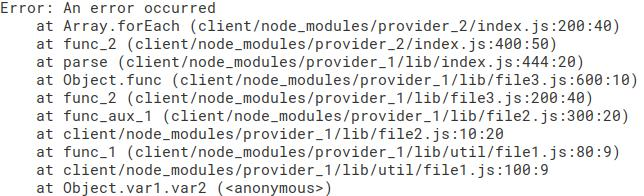
\includegraphics[scale=0.7]{figuras/stack_trace.jpeg}
    \caption{Generic stack-trace}
    \label{fig:trace}
\end{figure}{}

The stack trace is the base to analyze and an error.
All releases of any package that broke in the \textit{npm install} or \textit{npm test} were analyzed manually. The first step to analyze an error is differentiated between an error that wasn't caused by any provider, which is an error that occurred exclusively in the client package where the providers didn’t influence, and a breaking change error, that the errors occurred in provider package and it broke a client. There are two ways to conduct this step.

The first way is to take a look at the stack trace of the error and verify the calls to providers. When in the stack trace there isn't called to any providers, the error probably doesn’t refer a breaking change, because any provider was called in this error. So, the error is in the client code. To confirm this, the next commit in GitHub, after the release of the client, is verified. The objective is to verify if the error was fixed in any client commit. If true, the error is confirmed as a non-breaking change.
Some types of errors can be resolved in the code of the client. This error isn’t breaking change. Errors like \textit{SyntaxError} and \textit{ReferenceError}, where the client wrote the wrong code. Example:

\begin{lstlisting}[style=Javascript, label=cod:syntax:error, caption={Reference Error code in JavaScript}]
const a = 0 = 0;
\end{lstlisting}


In these errors, the npm raises a \textit{ReferenceError}. If the error is in the client code, nor is it necessary to look at \textit{GitHub}, because, for sure, the error is a non-breaking change. So, the code was fixed and the \textit{npm install} or \textit{npm test} is executed again to verify if any other error appeared.

The second way is when the errors can be a breaking change. This often occurs when the stack trace contains calls to any providers. However, providers like \textit{Mocha, Istanbul, Jasmine} and so on, that is, test frameworks, and task runners, like \textit{Grunt}, it is shown in stack trace but usually has no errors, because they only execute the files to test/tasks. So, when one of these providers is at the bottom of the stack tracer, they just called/execute the files/providers that contain the errors. Then, there’s a high probability that this error is a breaking change and this error can be caused by any provider.
To confirm this, the best place is in the \textit{GitHub}. The repository of the package contains all the information about the development. There are many ways to retrieve information. The easiest and most reliable way is to verify in a changelog file. These files, in general, are the \textit{CHANGELOG.md}, \textit{HISTORY.md} and others like this. These files contain the description of all changes about all packages releases. And many breaking changes are described there. For example, the release 5.0.0 of \textit{Mocha} contains a breaking change and was documented in \textit{CHANGELOG.md}. Figure \ref{fig:bc_documentation} show this documentation.

\begin{figure}
    \centering
    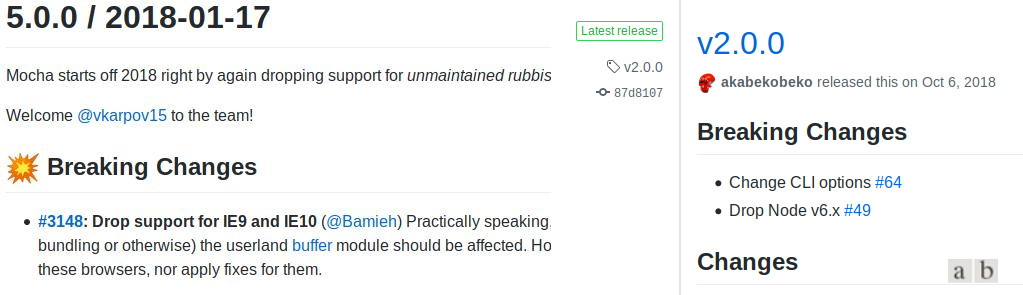
\includegraphics[scale=0.55]{figuras/bc_documentation.jpeg}
    \caption{Breaking Change documentation in README}
    \label{fig:bc_documentation}
\end{figure}{}

Other types of changelogs are the release notes. These are found in the comments of release. However, many and many repositories don’t contain a changelog file. Then, the next step is the search for any issue that contains some information about the error. In general, the issues contain much information, because of the developers and the owners of the package comment about the error. And more, many related issues are linked, increasing the number of information. Also, pull request works in the same way as issues.

Another important way is to install another release of the provider. So, it's possible to find out from which release the error started or which release the error was fixed. Also, there are other ways to verify if the error is in the provider. This is, compare the diff code between two provider releases; verify the provider commits; and change provider code.
The Figure \ref{fig:step_analyze} show a summary of these steps.

\begin{figure}
    \centering
    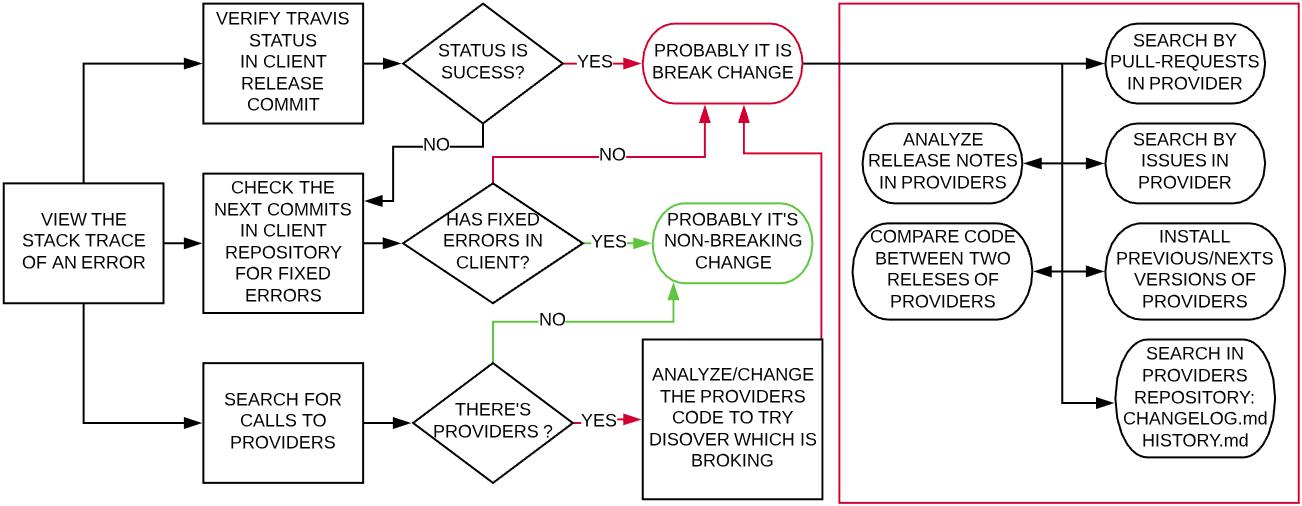
\includegraphics[scale=0.35]{figuras/step_analyze.jpeg}
    \caption{Steps to analyze an error}
    \label{fig:step_analyze}
\end{figure}
Some integrated systems can help to discover breaking changes. These systems are \textit{Travis, Jenkins, Codeship, CircleCI} and so on, and store the results of the npm install and npm test in the moment of a commit. It can help in the following way: if in the commit of a release the status of npm install or npm test was a success, and now is an error, then it occurred by a provider because the code of client is the same in the working tree and only the provider code was updated. However, just some of the sorted packages contain an integrated system.

Another detail is the packages that connect with some type of service likes, \textit{MySql, CouchDB, Redis} and so on. From all 385 packages, x required one of these services. When the \textit{npm install} or \textit{npm test} raises an error because of the connection, in manual analyze the required services were ability and re-executed the package. So, if the error was persister because the connection, the package was classified was \textit{Undiscovered Error}.

So, from all release analyze was saved many informations:

\begin{enumerate}
    \item Documentation about the error: issue, changelog, pull-request and so on;
    \item Who fixed the error: client or provider;
    \item How long did the error take to get fixed;
    \item Fixed in major, minor or patch; and
    \item In how many releases the error existed.
\end{enumerate}{}

Nor all information may be recovered. For example, if an error wasn't fixed, then neither the client nor the provider repaired the error.

\begin{itemize}
    \item RQ2: What issues in the provider package cause the manifestation of a breaking change?
\end{itemize}

For each error in \textit{npm install} or \textit{npm test}, it was manually analyzed. The objective is to do a grouping of similar errors and categorize then. For example, Figure \ref{fig:error_category} shows two errors in which one a function was renamed and the client tries to access the previous name.

\begin{figure}[!h]
    \centering
    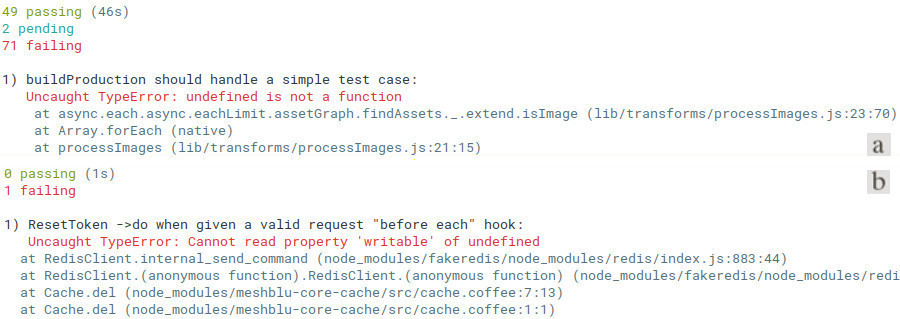
\includegraphics[scale=0.5]{figuras/error_category.jpeg}
    \caption{Two error caused by a renamed function}
    \label{fig:error_category}
\end{figure}

The first error in the Figure \ref{fig:error_category} is obvious: the client tries to access a variable like a function when it isn't a function. The second error talks about a property \textit{writable} that is access by an undefined object. There isn't any information about the function-related error, but, in manually analyze, it was observed that the provider change the name of a function. For this, in this code, the variable \textit{this.stream.writable} is undefined.

Once the provider causing the \textit{breaking change} has been discovered, there are several ways to find out the real reason that caused the error. These ways are described in Section \ref{cap:metodologia}. Then, all \textit{breaking changes} are classified based on his type.

\begin{itemize}
    \item RQ3: How do client packages recover from the manifestation of breaking change?
\end{itemize}

Since the customer recovers from the error, there are two ways to know how it recoverer. The first way is when the provider fixes his code and the client just updates the string of versioning in \textit{package.json}, if it needs. To the provider fixes the error, one issue may be done in his repository. The second way is when the client must do some work to fix the code. In this case, the client can fix the provider code and do a pull-request or change his code to work with the provider. And of course, may have cases that anyone does nothing. There is a breaking change and it’s never been fixed.

Where information about this RQ is retrieved is \textit{GitHub}. This information can be found at \textit{CHANGELOG, release-notes, issues,} and \textit{pull-requests}. If the \textit{changelog} contains information about fixed errors, in general, the related \textit{issues} are marked. From these \textit{issues}, a lot of more information can be recovered, like \textit{pull-requests} that are also marked in the \textit{issue}, other \textit{issues}, commentaries and more. All of this information can help us to discover which one -- client or provider -- fixed the \textit{breaking change} and how it was fixed.

\textit{Commits} are the alternative to \textit{issues} when the search is in the client repository. The \textit{commits} contain all changes in files and the all updates providers in \textit{package.json}. Commits message like \textit{update dependencies, fix dependencies, fix errors} an so on, suggests that something about any dependencies was fixed. This information is very important, because, since the provider was fixed and the client just updates it, the commit messages can tell the reason for this update - or downgrade.

%---------------------------------------------------%
\section{Considerações Finais}
\label{cap:metodologia:sec:consideracoes:finais}

Esta é uma sugestão de seção para dar um fechamento em cada uma dos capítulos.

(ATENÇÃO - veja com o seu orientador se é uma seção necessária (pois trate-se de estilo de escrita)) % Esse capítulo e nome é apenas uma sugestão.
%% ATENÇÃO - veja com o seu orientador se você vai ter este capítulo e se este vai ter nome!
\chapter{Experimentos e Resultados} 
\label{cap:experimentos:resultados}

Texto de ligação/introdução do capítulo...

(ATENÇÃO - veja com o seu orientador se você vai ter este capítulo e se este vai ter nome!)

%sugestão de seção
\section{Experimentos}
\label{cap:experimentos:sec:resultados:experimentos}

Descreva os experimentos realizados...

%sugestão de seção
\section{Resultados}
\label{cap:experimentos:resultados:sec:resultados}

Aqui você pode descrever os resultados obtidos nos experimentos e/ou analisar/discutir tais resultados.

%---------------------------------------------------%
\section{Considerações Finais}
\label{cap:experimentos:resultados:sec:consideracoes:finais}

Esta é uma sugestão de seção para dar um fechamento em cada uma dos capítulos. % Esse capítulo e nome é apenas uma sugestão.
%\chapter{Conclusões}
\label{cap:conclusoes}
 % Esse capítulo e nome é apenas uma sugestão.
\chapter{Draft}

\section{RQ1. Com que frequência \textit{breaking changes} surgem nos pacotes clientes?}
\label{sec:rq1}

\subsection{Motivação}
\label{mot:rq1}

No ecossistema do \gls{NPM}, uma simples \textit{release} que contenha um erro pode afetar uma quantidade imensa de pacotes, uma vez que este repositório contém a maior rede de dependências entre pacotes \cite{teorical_reference:npm_2}. Para evitar que \textit{breaking changes} se manifestem nos pacotes clientes, os provedores introduzem as \textit{breaking changes} em \textit{releases major}, seguindo o padrão do Versionamento Semântico, e os cliente podem utilizar \textit{strings semver} para aceitar apenas as versões \textit{minor} e \textit{patch} dos provedores -- o que é o padrão do \gls{NPM}. Entretanto, nem sempre o provedor é capaz de distinguir se suas alterações são \textit{breaking} ou \textit{non-breaking changes} \cite{noregrets2018}, ou, muitas vezes, as \textit{breaking changes} são introduzidas sem que o provedores percebam. Portanto, quando as \textit{breaking changes} são introduzidas em \textit{releases minor} ou \textit{patch}, elas podem causar comportamentos inesperados no cliente. Nesta RQ, será quantificado as manifestações das \textit{breaking changes} nos pacotes clientes. Assim, entender a frequência que os provedores publicam \textit{breaking changes} que afetam os clientes pode ajudar os clientes a fazer decisões melhores sobre como e quando atualizar a versão do seu provedor.

\subsection{Método}
\label{apr:rq1}

%\Gls{NPM}.
Um \textit{stack trace} é utilizado pelo \gls{NPM} para apresentar informações sobre um determinado erro. Quando os comandos \textit{npm install} e \textit{npm test} resultam em erro, o \Gls{NPM} mostra o erro e todas as chamadas de funções, incluindo as invocações para os provedores. A Figura \ref{fig:trace} mostra um exemplo genérico de um \textit{stack trace} exibido pelo \Gls{NPM}. Nesta Figura, no topo do \textit{stack trace}, contém o tipo do erro que interrompeu a execução e a sua mensagem. Nas linhas abaixo, há todas as funções e arquivos que foram executados até a manifestação do erro. Com todos estes dados, o \textit{stack trace} auxiliou no rastreamento de cada erro, uma vez que ele foi utilizado para detectar as \textit{breaking changes}, pois através do \textit{stack trace} foi possível identificar com exatidão em qual pacote o erro se manifestou: no ciente ou no provedor.

\begin{figure}
    \centering
    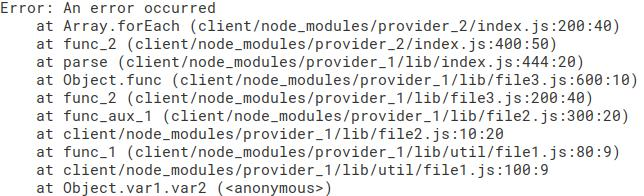
\includegraphics[scale=0.7]{figuras/stack_trace.jpeg}
    \caption{\textit{stack-trace} genérico}
    \label{fig:trace}
\end{figure}{}

Para quantificar as \textit{breaking changes}, foi necessário diferenciar entre um erro que foi causado pelo próprio pacote cliente, no qual não houve influência de nenhum provedor, e um erro que foi causado por algum dos provedores, sendo assim uma \textit{breaking change}. Esta diferenciação é necessária pois um determinado erro pode ter ocorrido no código do cliente e não em um provedor, assim não sendo um caso de \textit{breaking change}. Para realizar esta diferenciação, foi utilizado as seguintes heurísticas:

\begin{itemize}
    \item Verificar no \textit{stack trace}:
    \begin{itemize}
        \item quando não houve registros de execução dos provedores no \textit{stack trace}, provavelmente o erro não foi causado por uma \textit{breaking change}. Assim, o erro podia estar apenas no código do cliente; e

        \item quando houve registros de execução dos provedores no \textit{stack trace}, o erro provavelmente se tratava de uma \textit{breaking change}. Entretanto, as chamadas para \textit{frameworks} de teste, como o \textit{Mocha\footnote{https://www.npmjs.com/package/mocha}, Jasmine\footnote{https://www.npmjs.com/package/jasmine}} entre outros, ou automatizadores de tarefas, como o \textit{Grunt\footnote{https://www.npmjs.com/package/grunt}} por exemplo, não evidenciavam, inicialmente, a presença de \textit{breaking changes} uma vez que eles apenas iniciam a execução do pacote. Porém, não foi descartada a hipótese deles apresentarem \textit{breaking changes}.
    \end{itemize}{}

    \item  Próximos \textit{commits} do cliente: foi verificado no \textit{GitHub} se o cliente tentou consertar algum erro após a \textit{release} que apresentou o erro. Se foi encontrado algum \textit{commit} com correções, foram feitas estas alterações no código do cliente para verificar se as modificações encontradas no \textit{GitHub} realmente refletiam a correção do erro. Assim, se as alterações apenas no código do cliente refletiam na correção do erro, sem que haja influência dos provedores, então o erro não se tratava de uma \textit{breaking change};

    \item Sistemas integrados ao \textit{GitHub}: alguns sistemas integrados ao \textit{GitHub} auxiliaram na investigação. Esses sistemas são o \textit{Travis\footnote{https://travis-ci.org}, Codeship\footnote{https://codeship.com}} entre outros, que armazenam os resultados da execução do pacote para cada \textit{commit}. Eles foram utilizados da seguinte maneira: se nesses sistemas integrados, a execução no \textit{commit} da \textit{release} do cliente foi realizado com sucesso e, ao executá-lo nesta pesquisa, resultou em erro, significa que houve uma \textit{breaking change}, uma vez que o código do cliente estava na mesma \textit{working tree} do \textit{commit}. Mas, se a execução do cliente no momento do \textit{commit} resultou em erro, provavelmente os próximos \textit{commits} contêm alguma informação sobre o erro e sua correção, uma vez que estes sistemas integrados avisaram os desenvolvedores sobre o erro na execução.
\end{itemize}{}

Portanto, cada erro foi analisado manualmente, com alterações no código do cliente, para certificar se o erro era uma \textit{non-break change} ou uma \textit{break change}. Esta separação foi importante para esta e para as próximas questões de pesquisa. Com isto, foi quantificado os casos \textit{breaking changes} por \textit{releases}.


\subsection{Resultados}
\label{fin:rq1}

\subsubsection{De todos os pacotes, 11\% foram impactados por \textit{breaking changes}}

\subsubsection{Dos pacotes afetados, 13\% apresentaram mais de uma \textit{breaking change}}

\subsubsection{22\% das \textit{breaking changes} foram causadas por provedores indiretos}

\subsubsection{Os maiores provedores causaram mais \textit{breaking changes}}

%---------------------------------------------------%
\section{RQ2. Como os pacotes provedores introduzem \textit{breaking changes} em uma \textit{release}?}
\label{sec:rq2}

\subsection{Motivação}
\label{mot:rq2}
Pesquisas anteriores apresentam estudos sobre \textit{breaking changes} no ecossistema do \gls{NPM}. Entretanto, pelo fato do \textit{Javascript} ser dinâmico, estes estudos focaram apenas nas alterações de \gls{API}, tais como as remoções/renomeações, alterações na lista de parâmetros e alterações no tipo de retorno. Estes estudos foram realizados por  \citeonline{teorical_reference:bc_1} e \citeonline{noregrets2018} e não verificaram \textit{breaking changes} além das relacionadas às \gls{API}. Desta maneira, além das alterações em \gls{API}, não se tem informações sobre como os provedores introduzem \textit{breaking changes}, ou seja, quais os principais casos que fazem com que o cliente sofra uma \textit{breaking changes}. Por causa da falta de informação, muitas \textit{breaking changes} são introduzidas, mas poderiam ser facilmente evitadas. Assim, grande parte das \textit{breaking changes} em \textit{JavaScript} são detectadas apenas em tempo de execução \cite{noregrets2018}, mas para o cliente, ter seu código encerrado em tempo de execução pode ser muito custoso. Por isso, dimensionar e categorizar as \textit{breaking changes} ajudará os desenvolvedores a atentar-se para as \textit{breaking changes} mais comuns e tentar evitá-las, assim produzindo códigos menos favoráveis às \textit{breaking changes}.

\subsection{Método}
\label{apr:rq2}

O objetivo da análise manual é descobrir o motivo que originou uma \textit{breaking changes}, ou seja, qual foi a alteração que o provedor realizou que causou a \textit{breaking change} para que seja possível agrupa-las por suas similaridades. A análise manual é essencial, pois o \textit{stack trace} sempre apresenta o erro de uma maneira genérica. Então, as vezes, a mensagem de erro pode induzir a interpretação errônea do real motivo que originou a falha.

Cada caso de \textit{breaking change} será analisado e motivo que levou a sua manifestação será anotado para ser comparado com os demais. Após descobrir que um erro diz respeito à alteração de \gls{API}, por exemplo, uma categoria chamada \textit{Função Renomeada} será criada e as demais \textit{breaking changes} que possuem características comuns a esta também serão categorizadas como \textit{Função Renomeada}. Assim será possível quantificar cada uma das categorias. E mesmo processo será realizado para as demais \textit{breaking changes}, sempre visando criar categorias da maneira mais genérica que agrupe os erros semelhantes.

\subsection{Findings}
\label{fin:rq2}

%---------------------------------------------------%
\section{RQ3. Como os pacotes clientes se recuperam das breaking change?}
\label{sec:rq3}

\subsection{Motivação}
\label{mot:rq3}
Uma vez que uma \textit{breaking change} é introduzida, o cliente deve se recuperar dessa. Isso se faz necessário pois, no ecossistema \gls{NPM}, no qual centenas de milhares de pacotes estão conectados, uma simples \textit{release} com erro pode ocasionar na quebra de muitos clientes. No entanto, como os provedores evoluem independentemente dos clientes, erros e vulnerabilidades são difíceis de rastrear e corrigir nos clientes. Mesmo quando as vulnerabilidades podem ser corrigidas com a atualização para uma versão mais recente do provedor, pode haver incompatibilidades de \textit{API} -- entre outras incompatibilidades -- com os clientes que deve ser resolvido manualmente \cite{Foo:2018:ESC:3236024.3275535}. Desta maneira, entender como o cliente reage às \textit{breaking changes} ajudará os próprios clientes e os provedores a conhecerem as alternativas frente a uma \textit{breaking change} para que os clientes possam se recuperar da maneira mais eficiente.

\subsection{Método}
\label{apr:rq3}
Uma vez que os clientes se recuperaram de um erro, há duas maneiras para se obter informações sobre esta recuperação. A primeira maneira é quando o provedor corrige seu código e o cliente apenas atualiza sua \textit{string} de versionamento no \textit{package.json}, se precisar. Para o provedor consertar o erro, deve haver uma \textit{issue} no seu repositório. A segunda maneira é quando o próprio cliente conserta o código. Neste caso, o cliente pode corrigir o código do provedor e realizar um \textit{pull-request}. Também, o cliente pode alterar apenas o seu código para que execute normalmente com a \textit{release} errônea do provedor. Há casos também no qual nem o cliente nem o provedor faz nada para consertar o erro.

Todas as informações sobre esta questão de pesquisa foram recuperadas do \textit{GitHub}. As informações foram encontradas em \textit{CHANGELOGs, release-notes, issues} e \textit{pull-requests}. Os \textit{CHANGELOGs} contêm informações sobre os erros consertados. A partir das \textit{issues} é possível entender com os comentários dos clientes quais foram as ações que eles realizaram para se recuperar de uma determinada \textit{breaking change}. Pois, assim como o código de um pacote fica emaranhado com o código no restante do ecossistema ao qual ele pertence, o mesmo acontece com as \textit{issues}. Uma manifestação disso é que muitas \textit{issues} abertas em um projeto são vinculadas a \textit{issues} relacionadas, em projetos iguais ou diferentes, pois os desenvolvedores estão rastreando as causas de um problema \cite{Zhang:2018:WIL:3242887.3242891}. De maneira análoga, os \textit{pull-requests} que são relacionados ao mesmo problema também são marcados. Todas estas informações corroboram para descobrir como a \textit{breaking change} foi tratada/consertada e quem -- cliente ou provedor -- a consertou, caso tenha sido consertada.

Os \textit{commits} são alternativas para as \textit{issues} quando a busca se dá no repositório do cliente. Sobre os \textit{commits}, mensagens do tipo \textit{update dependencies, fix dependencies, fix errors} etc. sugerem que algum provedor foi atualizado para consertar algum erro ou um erro foi consertado diretamente no código do cliente. Esta informações é muito importante, uma vez que o provedor corrigiu a \textit{breaking change} e o cliente apenas o atualizou. Assim, as mensagens dos \textit{commits} auxiliaram para descobrir os reais motivos da atualização -- ou retrocesso da versão.

\subsection{Findings}
\label{d_fin:rq3}
 % Esse capítulo e nome é apenas uma sugestão.
\section{RQ1. Com que frequência \textit{breaking changes} surgem nos pacote clientes?}
\label{sec:rq1}

\subsection{Motivation}
\label{mot:rq1}

Atualmente, o \Gls{NPM} contém mais de 11 bilhões de downloads semanais e ultrapassa os 45 bilhões por mês. Os pacotes hospedados no \Gls{NPM} são usados por milhões de pessoas e projetos por todo o mundo. Eles são gratis, e fáceis de usar. Entretanto, uma simples \textit{release} que contenha um erro pode afetar uma quantidade imensa de pacotes. Isso se deve ao fato dos pacotes dependerem uns dos outros, direta ou indiretamente e, quando uma \textit{release} introduz \textit{breaking changes}, muitos pacotes podem ser afetados.

Para evitar estes erros, o \Gls{NPM} utiliza \textit{strings} de versionamento, baseadas no \Gls{SEMVER} para especificar as versões dos provedores. Isso permite que um provedor publique uma \textit{release} que contenha \textit{breaking changes}, mas que não afete os clientes das versões prévias. Entretanto, pesquisas mostram que a distinção entre \textit{breaking} e \textit{non-breaking changes} não é totalmente clara e pode ser difícil para o desenvolvedor decidir como incrementar a \textit{string} de versionamento a cada \textit{release} \cite{noregrets2018}. Assim sendo, entender com que frequência os pacotes provedores publicam \textit{releases} com \textit{breaking changes} pode ajudar os clientes a fazerem uma decisão melhor sobre como e quando atualizar a versão do provedor.

Para responder essa questão de pesquisa, serão analisados três pontos: 1) quantas vezes cada provedor publica uma \textit{release} que contém \textit{breaking changes} - e qual é a porcentagem de \textit{releases}; 2) em qual nível da \textit{string} de versionamento as \textit{breaking changes} são tipicamente introduzidas, de acordo com o \Gls{SEMVER} - \textit{major, minor} ou \textit{patch}; 3) qual o percentual de clientes que atualizam para uma versão com \textit{breaking changes}.

Para analisar todos esses pontos, os pacotes sorteados foram clonados do \textit{GitHub}, atualizado o \textit{index} e os arquivos na \textit{Working Tree} através do comando \textit{git checkout} com o \textit{timestamp} da \textit{release}, excluido o arquivo \textit{package-lock.json}, atualizado a versão de cada um dos provedores no \textit{package.json} e executado os comandos \textit{npm install} e \textit{npm test}. Todo esse processo foi executado automaticamente pela ferramenta \textit{BCDetect} \footnote{https://github.com/danielventurini/bcdetect}. Então, o resultado da execução -- sucesso ou erro -- foi salvo juntamente com as informações sobre a versão do \textit{Node.JS} que foi executado e que deveria ter sido executada, de acordo com o \textit{timestamp}. % essa parte das versões eu vou explicar melhor em um capítulo falando sobre a ferramenta.

\subsection{Approach}
\label{apr:rq1}
Um \textit{stack trace} contém as informações sobre as subrotinas de um programa. É comumente utilizado para certos tipos de \textit{debugs}, nos quais eles auxiliam a visualizar e rastrear um determinado evento/erro. Quando os comandos \textit{npm install} e \textit{npm test} resultam em erro, o \Gls{NPM} mostra o erro e todas as chamadas de função, incluindo as invocações para os provedores. A Figura \ref{fig:trace} mostra um exemplo genérico de um \textit{stack trace} mostrado pelo \Gls{NPM} após a ocorrência de um erro.

\begin{figure}
    \centering
    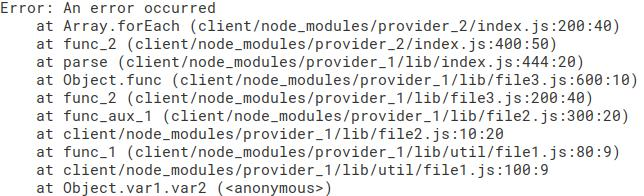
\includegraphics[scale=0.7]{figuras/stack_trace.jpeg}
    \caption{Generic stack-trace}
    \label{fig:trace}
\end{figure}{}

O \textit{stack trace} é a base para analisar um erro. A primeira etapa da análise de um erro é diferenciar entre um erro que foi causado pelo próprio pacote cliente, no qual não houve influência de nenhum provedor, portanto não caracteriza uma \textit{breaking change}, e um erro que foi causado por algum dos provedores, no qual se propagou para o pacote cliente e interrompeu-lhe a execução. Há duas maneiras que foi utilizada para realizar esta análise.

A primeira maneira foi verificar diretamente no \textit{stack trace} do erro e procurar as chamadas de função para os provedores. Quando não há chamada para os provedores no \textit{stack trace}, provavelmente o erro não se trata de uma \textit{breaking change}, porque nenhum provedor influenciou em nada na execução até acontecer o erro. Então, a falha pode estar apenas no código do cliente. Para confirmar isto, foi procurado no \textit{GitHub} do cliente os próximos \textit{commits} e verificado se o desenvolvedor realizou alguns \textit{commits} com a intenção de consertar algum erro - mensagens do tipo \textit{fix error}, \textit{fix bugs} etc. Se sim, o código do cliente foi alterado para verificar se as modificações presentes nos \textit{commits} realmente refletem a correção do erro. Então este caso foi confirmado como um \textit{non-breaking change} e foi descartado. Entretanto, alguns tipos de erros já indicam exatamente onde o erro aconteceu. São os \textit{SyntaxError} e \textit{ReferenceError}, no qual já se sabe onde e porque ocorreu. O Código \ref{cod:syntax:error} mostra um exemplo deste tipo de erro.

\begin{lstlisting}[style=Javascript, label=cod:syntax:error, caption={Código com um Reference Error}]
const a = 0 = 0;
\end{lstlisting}

Nesses casos, no qual o erro estava no pacote cliente, nem se fez necessário procurar por \textit{commits} no \textit{GitHub}. Apenas foi consertado diretamente no código do cliente e re-executado o comando que resultou em erro: \textit{install} ou \textit{test}. Isto para garantir que não houvesse um segundo erro que pudesse ser uma \textit{breaking change}.

A segunda maneira é quando o erro indicava a presença de \textit{breaking changes}. Isto se evidenciava quando havia chamadas para os provedores no \textit{stack trace}. Entretanto, as chamadas para \textit{frameworks} de teste, como o \textit{Mocha, Instanbul, Jasmine} entre outros, ou automatizadores de tarefas, o \textit{Grunt} por exemplo, não evidenciam diretamente a presença de \textit{breaking changes} uma vez que eles apenas iniciam a execução do pacote e deveriam estar ali. Porém, não foram totalmente descartados de apresentar \textit{breaking changes}. Assim, quando havia algum provedor no \textit{stack trace}, provavelmente se tratava de um caso de \textit{breaking change}.

O melhor local para se confirmar esta evidência é o \textit{GitHub}. Neste, os repositórios dos pacotes contêm todo o histórico de desenvolvimento. E muitas maneiras foram utilizadas para recuperar as informações necessárias. A primeira e mais fácil foi procurar nos arquivos registros de alterações, os comumente nomeados de \textit{CHANGELOG.md} ou \textit{HISTORY.md}. A proposta destes arquivos é manter uma lista ordenada cronologicamente das alterações significativas ao longo do desenvolvimento do projeto. E uma das informações muito importantes que são descritas nesses registos são as \textit{breaking changes}. Por exemplo, a versão \textit{5.0.0} do projeto \textit{Mocha} \footnote{https://github.com/mochajs/mocha} contém uma \textit{breaking change} que foi documentada no \textit{CHANGELOG.md}\footnote{https://github.com/mochajs/mocha/blob/master/CHANGELOG.md\#500--2018-01-17}. A Figura \ref{fig:bc_documentation} ilustra como foi realizada esta documentação.

\begin{figure}
    \centering
    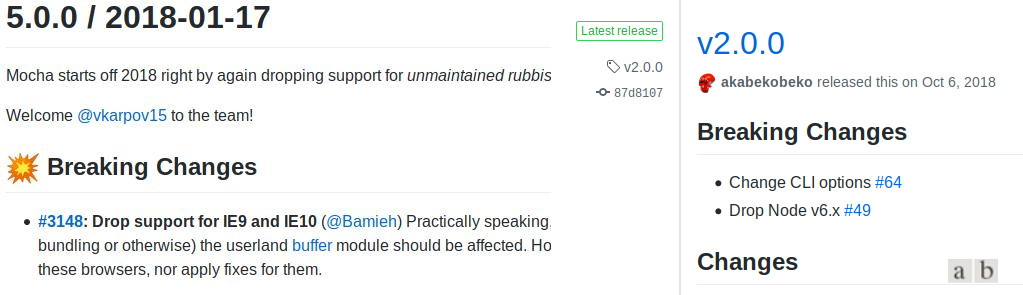
\includegraphics[scale=0.55]{figuras/bc_documentation.jpeg}
    \caption{Breaking Change documentation in README}
    \label{fig:bc_documentation}
\end{figure}{}

Assim, foi observado a versão do provedor que possivelmente causou o erro e foi verificado no seu \textit{CHANGELOG} -- caso existisse -- se contém alguma informação pertinente ao erro que foi apresentado pelo \gls{NPM} quando resultou em erro. Então foi salva as informações sobre este erro: a versão que iniciou, a versão que foi corrigido, uma breve descrição para facilitar a classificação da \textit{breaking change}, quem consertou o erro: cliente ou provedor; o tempo total até ser corrigido, quantas \textit{releases} o provedor levou para corrigir e em qual nível do \gls{SEMVER} o erro foi consertado.

Há ainda outros tipos de documentações parecidas com os \textit{changelogs}. Uma delas são as \textit{releases notes}. Elas são observações importantes sobre as alterações introduzidas por cada \textit{release}. Além disso, foi verificado nas \textit{issues} dos repositórios. Lá, muitas informações foram encontradas. E muito mais, pois há uma grande rede interligada de \textit{issues} e \textit{pull-requests} no qual uma \textit{issue} é marcada em outra \textit{issue}, que é marcada em um \textit{pull-request} e assim por diante. Deste modo, uma simples \textit{issue}/\textit{pull-request} contém muita informação.

Um ponto que foi muito importante para descobrir as versões que foram introduzidas as \textit{breaking changes} é a instalação de versões prévias e sucessivas dos provedores. Com isso, foi possível testar a partir de qual versão o erro foi introduzido e consertado e descobrir qual foi o verdadeiro provedor causador do erro. Também, alguns outros recursos foram utilizados para buscar as informações desta questão de pesquisa, tais como, o uso da ferramenta \textit{npm-diff}\footnote{https://github.com/danielventurini/npm-diff}, que provê os \textit{diff} do código entre duas \textit{releases} de um determinado projeto, no qual foi verificado o que realmente foi introduzido e o que foi removido com mais detalhes.

A Figura \ref{fig:step_analyze} exemplifica as técnicas utilizadas para responder esta questão de pesquisa.

\begin{figure}
    \centering
    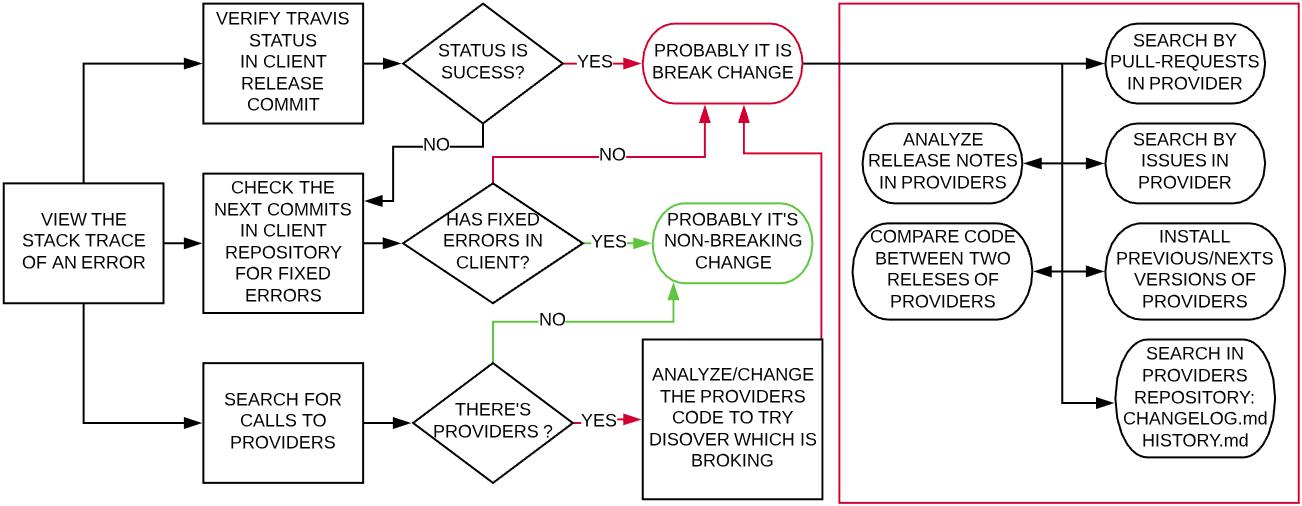
\includegraphics[scale=0.35]{figuras/step_analyze.jpeg}
    \caption{Passos para analisar um erro}
    \label{fig:step_analyze}
\end{figure}

Vale ressaltar que alguns sistemas integrados ao \textit{GitHub} auxiliaram na investigação. Esses sistemas são o \textit{Travis, Jenkins, Codeship, CicleCI} etc. que, quando o desenvolvedor realizou o \textit{commit}, esses sistemas executaram o \textit{npm install} e o \textit{npm test}. Isto colaborou da seguinte maneira: se o \textit{commit} da \textit{release} foi salvo o resultado do \textit{npm install} e \textit{npm test} como sucesso e, ao executá-los nesta pesquisa foi resultado em erro, indica que há uma \textit{breaking change}, uma vez que o código do cliente está no mesmo index do \textit{working tree}, apenas os provedores que foram atualizados e, para o range aceito, geraram erros, resultando em \textit{breaking changes}. Entretanto, nem todos os projetos utilizavam estes sistemas integrados, mas quando dispunham, foi de grande valia.

Outro detalhe importante se refere aos projetos que utilizavam algum tipo de sistemas terceiros como o \textit{MySql, CouchDB, Redis} etc. Então, quando foi gerado um erro pela falta de um destes, fez-se a habilitação destes e o pacote foi re-executado. Entretanto, quando os pacotes requeriam previamente uma configuração para executar, tais como a criação de tabelas em banco de dados, esta configuração foi feita, seguindo o modelo disponibilizado pelo desenvolvedor afim de realizar os teste, e novamente foi executado o pacote.

Então, para todas as \textit{releases} analisadas manualmente, foi salvo as seguintes informações:

\begin{enumerate}
    \item Em que local o erro foi documentado: \textit{issue, changelog, pull-request} etc;
    \item Quem consertou o erro: cliente ou providor;
    \item Em qual nível do \textit{SEMVER} o erro foi reparado;
    \item Quanto tempo o erro levou até ser corrigido; e
    \item Por quantas \textit{releases} o erro persistiu.
\end{enumerate}{}

\subsection{Findings}
\label{fin:rq1}

%---------------------------------------------------%
\section{RQ2. Quais são os problemas no pacote provedor que causam breaking change?}
\label{sec:rq2}

\subsection{Motivation}
\label{mot:rq2}

Uma vez que o provedor teve um comportamento inesperado pelo cliente, há \textit{breaking changes}. Isso pode causar uma mudança no comportamento do pacote cliente e, no pior caso, causar o encerramento de toda a execução se o cliente previamente na tratou um determinado erro. Entretanto, um cliente nunca espera que o provedor tenha um erro e, por isso, não fica tratando todas as chamadas para o cliente com \textit{try catch}. Assim, o cliente confia que o provedor esteja executando da maneira que foi especificado.

Um provedor pode conter múltiplos tipos de erros. Uma simples linha escrita semanticamente errada, por exemplo, pode causar no encerramento da execução, uma vez que os códigos \textit{Javascript} não são compilados. Entretanto, um erro pode não estar no provedor diretamente. Isto é devido ao fato deste contém um segundo provedor que seja o causador da \textit{breaking change}. Então, o erro é propagado do segundo provedor para o primeiro e, por fim, alcança o cliente. Isto é uma \textit{breaking change} transitiva e, na nossa pesquisa, é tratada como um caso normal de \textit{breaking change}.

Para responder essa questão de pesquisa, foi analisado caso a caso dos erros e as \textit{breaking changes} foram categorizadas pelo tipo da \textit{breaking change}. Também, os tipos foram quantificados pela categoria, pelo número de \textit{releases} afetadas e pelo número de clientes que sofreram com uma determinada categoria de \textit{breaking change}.

\subsection{Approach}
\label{apr:rq2}

Cada um dos casos de erro para os comandos \textit{npm install} e \textit{npm test} foram analisados manualmente. O objetivo era descobrir o real motivo que origino o erro e agrupa-los por suas similaridades. A Figura \ref{fig:error_category} mostra dois casos no qual uma função foi renomeada pelo provedor. Entretanto, previamente não está claro o real motivo dos erros, apesar da mensagem do \textit{stack trace}.

\begin{figure}[!h]
    \centering
    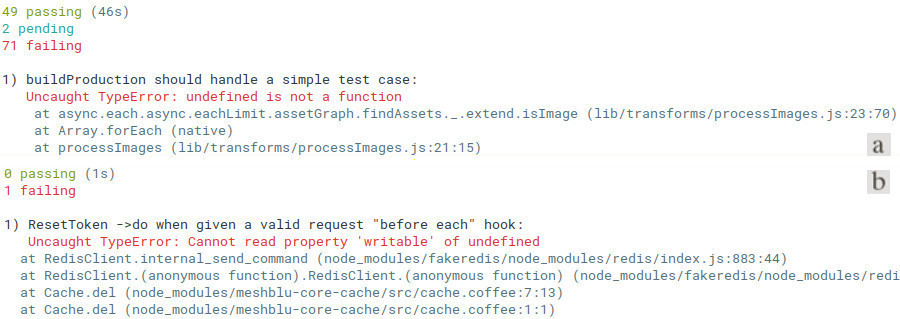
\includegraphics[scale=0.5]{figuras/error_category.jpeg}
    \caption{Two error caused by a renamed function}
    \label{fig:error_category}
\end{figure}

A mensagem do primeiro erro deixa claro que se trata de uma invocação a uma função inexistente, ou seja, o cliente tentou acessar uma variável como uma função quando esta não era. Mas, somente pela mensagem do \textit{stack trace} é possível deduzir que uma função foi renomeada no provedor. Já no segundo erro, o \textit{stack trace} não indica que o erro se trata de uma função renomeada. Somente após uma análise deste caso é que foi possível concluir que o erro aconteceu por uma função renomeada. Assim, apesar de mensagens de erro diferentes, foram classificados pelo seu real motivo para que fosse possível quantificar os principais problemas no código do provedor.

\subsection{Findings}
\label{fin:rq2}

%---------------------------------------------------%
\section{RQ3. Como os pacotes clientes se recuperam das breaking change?}
\label{sec:rq3}

\subsection{Motivation}
\label{mot:rq3}

Uma vez que uma \textit{breaking change} é introduzida o provedor deve se recuperar desta. Isso se faz necessário pois, no ecossistema \gls{NPM}, no qual centenas de milhares de pacotes estão conectados, uma simples \textit{release} com erro pode ocasionar na quebra de muitos clientes. Isto ocorreu com um pacote chamado \textit{left-pad}\footnote{https://blog.npmjs.org/post/141577284765/kik-left-pad-and-npm}. Este foi removido do \textit{NPM} por seu desenvolvedor e impactou milhares de projetos em apenas 2.5 horas incluindo \textit{babel}\footnote{https://github.com/babel/babel} e \textit{atom}\footnote{https://github.com/atom/atom}.

A responsabilidade para corrigir uma errônea \textit{release} é do provedor. Entretanto, as vezes, o provedor deixa dar a manutenção por algum motivo. Então, os clientes recebem esta responsabilidade, uma vez que o erro no seu provedor pode afetar os seus clientes. No caso do \textit{left-pad} o provedor nunca publicou uma nova \textit{release} e, para que todos os pacotes continuassem a executar normalmente, um dos clientes publicou um pacote com o mesmo nome e mesmo código, uma vez que a política para nomes de pacotes permitia este feito e o pacote original continha uma licença de código aberto.

Entretanto, nem sempre o cliente consegue resolver um problema no provedor. Isso se deve ao fato do cliente não ter conhecimento prévio do funcionamento interno do provedor ou por outros motivos. Assim, o cliente dificilmente irá conseguir ter sucesso quanto a resolução do erro no provedor. Então, uma alternativa para o cliente é alterar o seu provedor buscando por um que atenda as necessidades que não fora atendidas pelo provedor prévio.

Para responder a questão de pesquisa final, foi analisado três pontos: 1) o que aconteceu para que o provedor não pudesse consertar o erro; 2) como o cliente consertou o erro: no seu código ou notificando o provedor através de \textit{issues} e \textit{pull-requests}; 3) quantas vezes o cliente teve que realizar a correção dado que o provedor não a fez. Todas as informações sobre esta questão de pesquisa estão nos \textit{commits}, \textit{issues}, \textit{pull-requests}, \textit{changelogs} e \textit{releases-notes} dos repositórios do cliente e do provedor.

\subsection{Approach}
\label{apr:rq3}

Uma vez que os clientes se recuperaram de um erro, há duas maneiras para se obter informações sobre esta recuperação. A primeira maneira é quando o provedor corrige seu código e o cliente apenas atualiza sua \textit{string} de versionamento no \textit{package.json}, se precisar. Para o provedor consertar o erro, deve haver uma \textit{issue} no seu repositório. A segunda maneira é quando o próprio cliente conserta o código. Neste caso, o cliente pode corrigir o código do provedor e realizar um \textit{pull-request}. Também, o cliente pode alterar apenas o seu código para que execute normalmente com a \textit{release} errônea do cliente. Há casos também no qual nem o cliente nem o provedor faz nada para consertar o erro.

Where information about this RQ is retrieved is \textit{GitHub}. This information can be found at \textit{CHANGELOG, release-notes, issues,} and \textit{pull-requests}. If the \textit{changelog} contains information about fixed errors, in general, the related \textit{issues} are marked. From these \textit{issues}, a lot of more information can be recovered, like \textit{pull-requests} that are also marked in the \textit{issue}, other \textit{issues}, commentaries and more. All of this information can help us to discover which one -- client or provider -- fixed the \textit{breaking change} and how it was fixed.

\textit{Commits} are the alternative to \textit{issues} when the search is in the client repository. The \textit{commits} contain all changes in files and the all updates providers in \textit{package.json}. Commits message like \textit{update dependencies, fix dependencies, fix errors} an so on, suggests that something about any dependencies was fixed. This information is very important, because, since the provider was fixed and the client just updates it, the commit messages can tell the reason for this update - or downgrade.

\subsection{Findings}
\label{fin:rq3} % Esse capítulo e nome é apenas uma sugestão.

% Apendices.
%\appendix
%\chapter{Instalação de Ferramentas}
\label{ape:instalacao:ferramentas}

Os apêndices são usados para disponibilizar materiais extras que por questões de espaço ou estilo de escrita não foram colocados diretamente no texto. Por exemplo, \textit{scripts}, instruções de instalação das ferramentas utilizadas pelo trabalho, partes de código fonte e questionários que tenham sido aplicados, tabelas com resultados...

(ATENÇÃO - veja com o seu orientador se é necessário disponibilizar algum material extra sobre algum capítulo em anexo!)



%bibliografia
\bibliographystyle{abntex2-alf}
\bibliography{main} % geração automática das referências a partir do arquivo main.bib

%\backmatter
\end{document}
